\documentclass{beamer} 
%\usetheme{Boadilla} 
%\usetheme{CambridgeUS}
%\usetheme{Warsaw}
%\usetheme{Berkeley}
%\usetheme{Copenhagen}
%\usetheme{Berkeley}
%\usetheme{Malmoe}
%\usetheme{PaloAlto}
%usetheme{Pittsburgh}

\usecolortheme{rose}
\usetheme{Madrid}
\useinnertheme{circles} 
\newenvironment{conenv}{\only{\setbeamercolor{local structure}{fg=darkred}}}{} 
\setbeamercovered{dynamic} 
\setbeamertemplate{navigation symbols}{} 
\definecolor{links}{HTML}{2A1B81} 
\hypersetup{colorlinks,linkcolor=,urlcolor=links} 
\usepackage[utf8]{inputenc} 
\usepackage{eurosym} 
\usepackage{subfigure} 
\usepackage{graphicx} 
\usepackage{booktabs}
\usepackage{color} 
\usepackage{appendixnumberbeamer}

\title[W+Jets background Study]{W+Jets background Study}
\author[Raman Khurana]{Shin-Shan Yu, Fang-Ying Tsai, Ching-Wei Chen}% (optional, for multiple authors)
%\institute[National Central University, Taiwan]{

%\date[Group meeting]{\today}



\begin{document} 

\begin{frame} 

\titlepage 
\end{frame} 

\setbeamercolor{itemize item}{fg=blue}

\begin{frame}
\frametitle{Selection used for W+Jets Control region}
\begin{itemize}
%\item MET $>$ 200 GeV
\end{itemize}
\end{frame}


%
%
%\begin{frame}
%\frametitle{Efficiency(Single Electron Trigger with Different ID}
%\begin{center}                                                                                                                                
%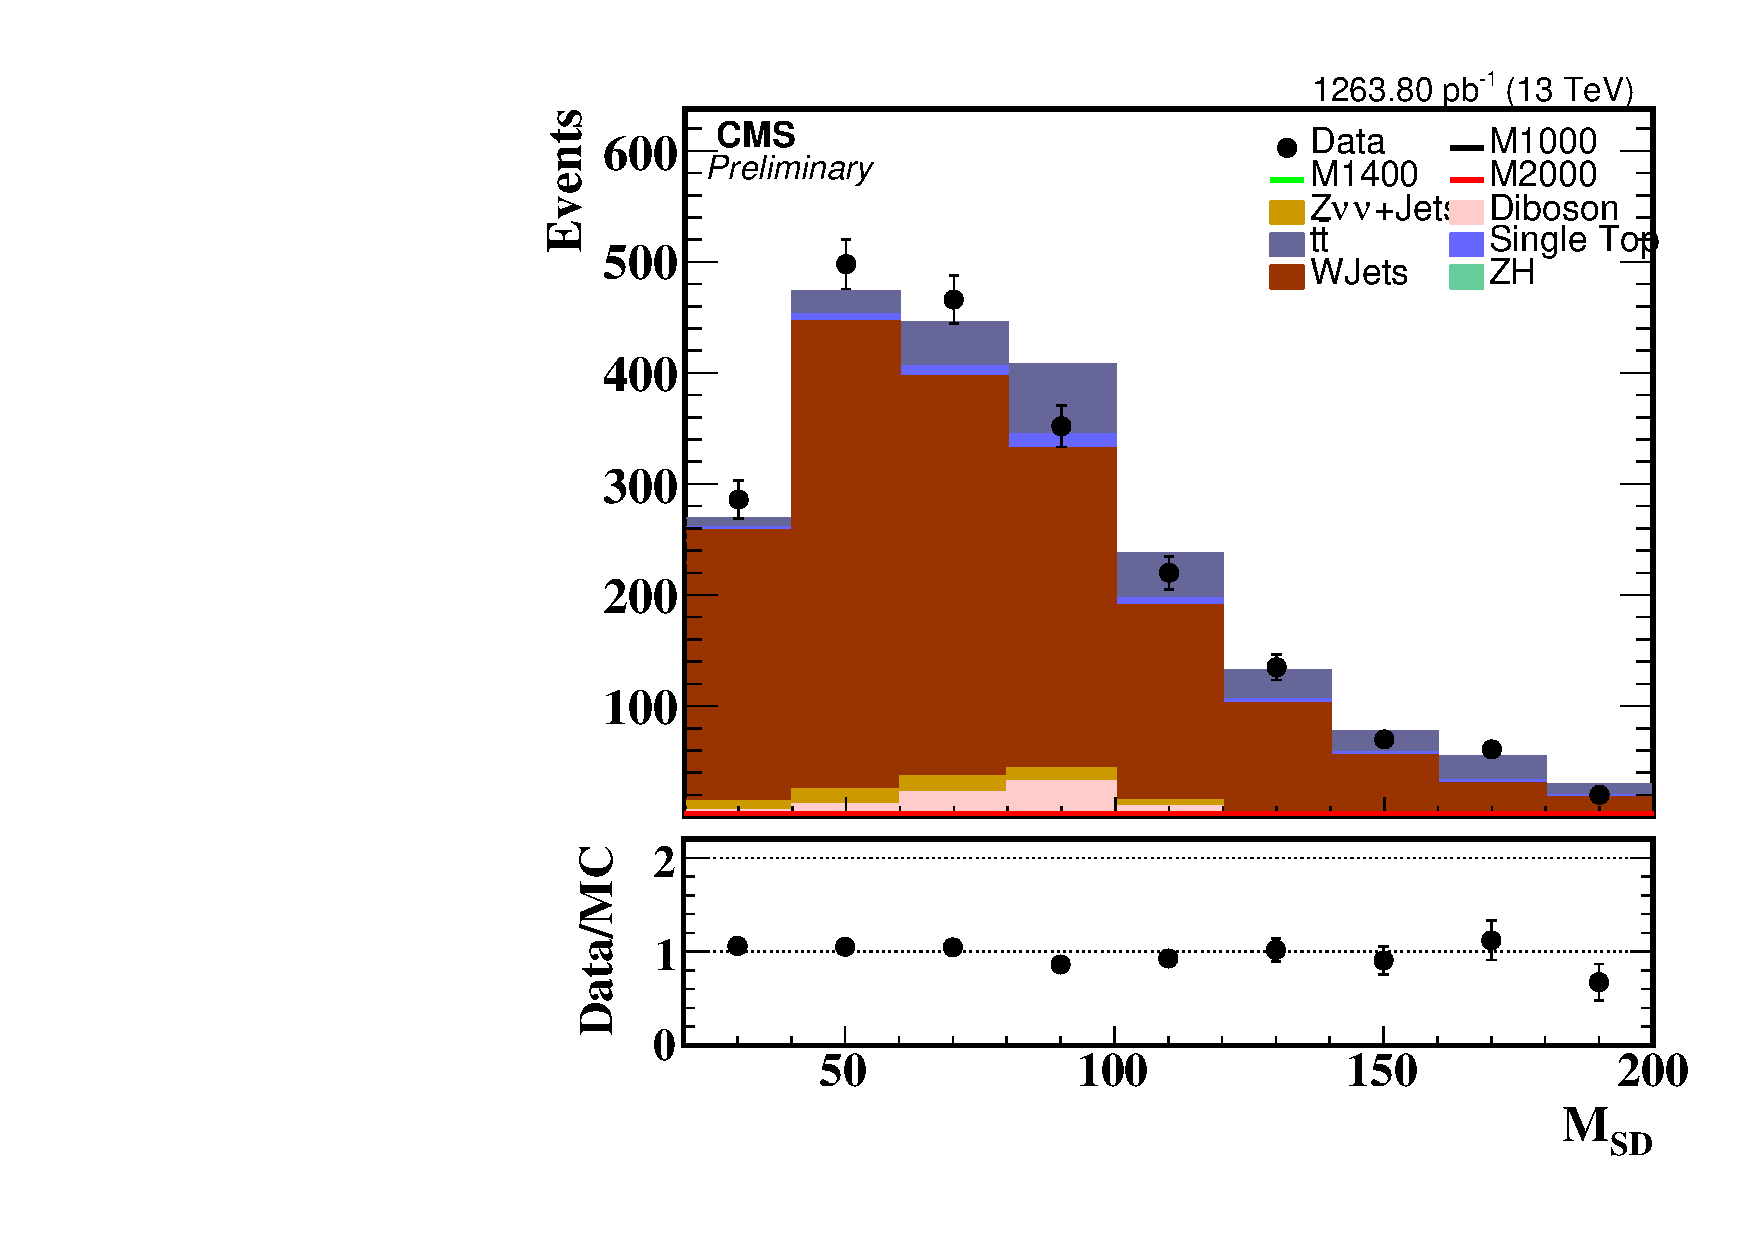
\includegraphics[angle=0,height=0.22\textwidth]{PlotsRaman_VeniceConf30112015/DYPdf/histfacFatJet_WLight_h_Mjj0.pdf}
%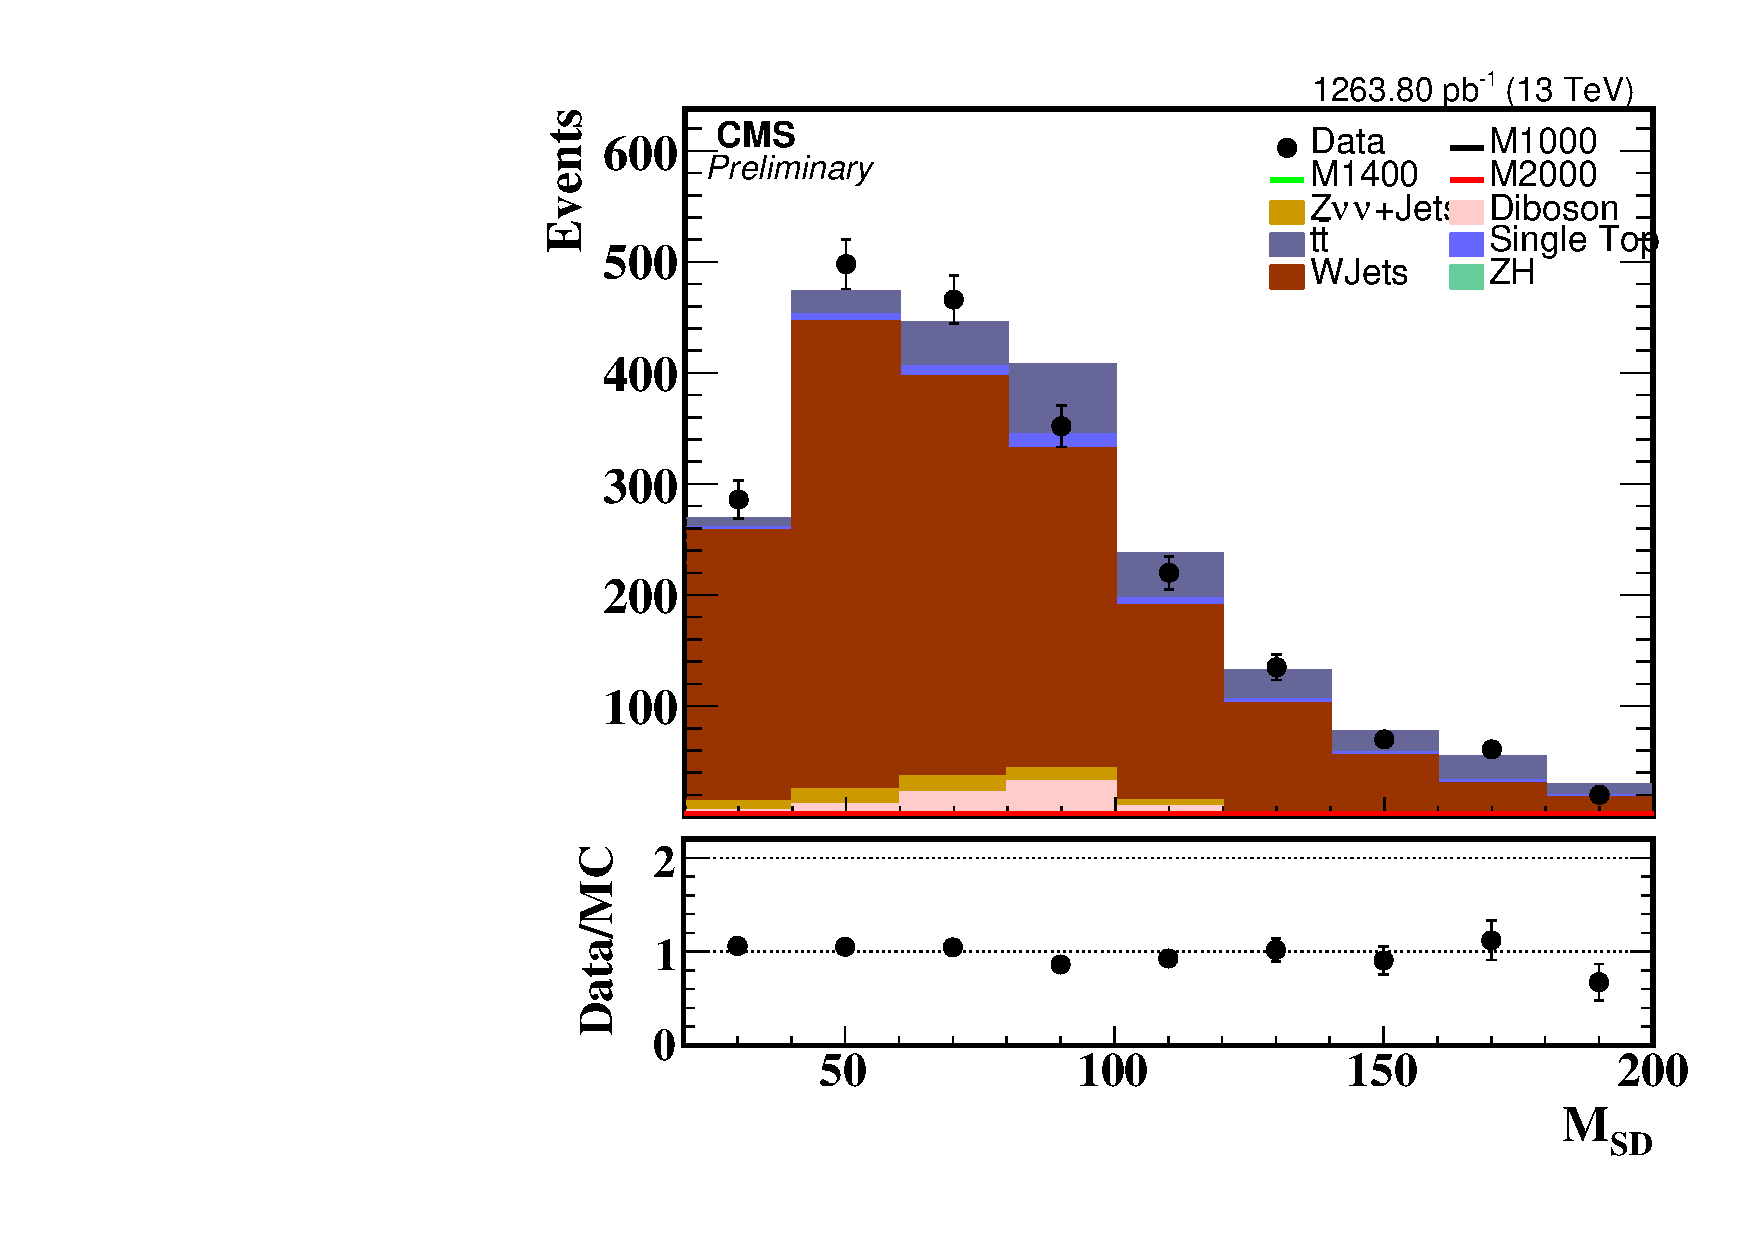
\includegraphics[angle=0,height=0.22\textwidth]{PlotsRaman_VeniceConf30112015/DYPdf/histfacFatJet_WLight_h_Mjj0.pdf}\\
%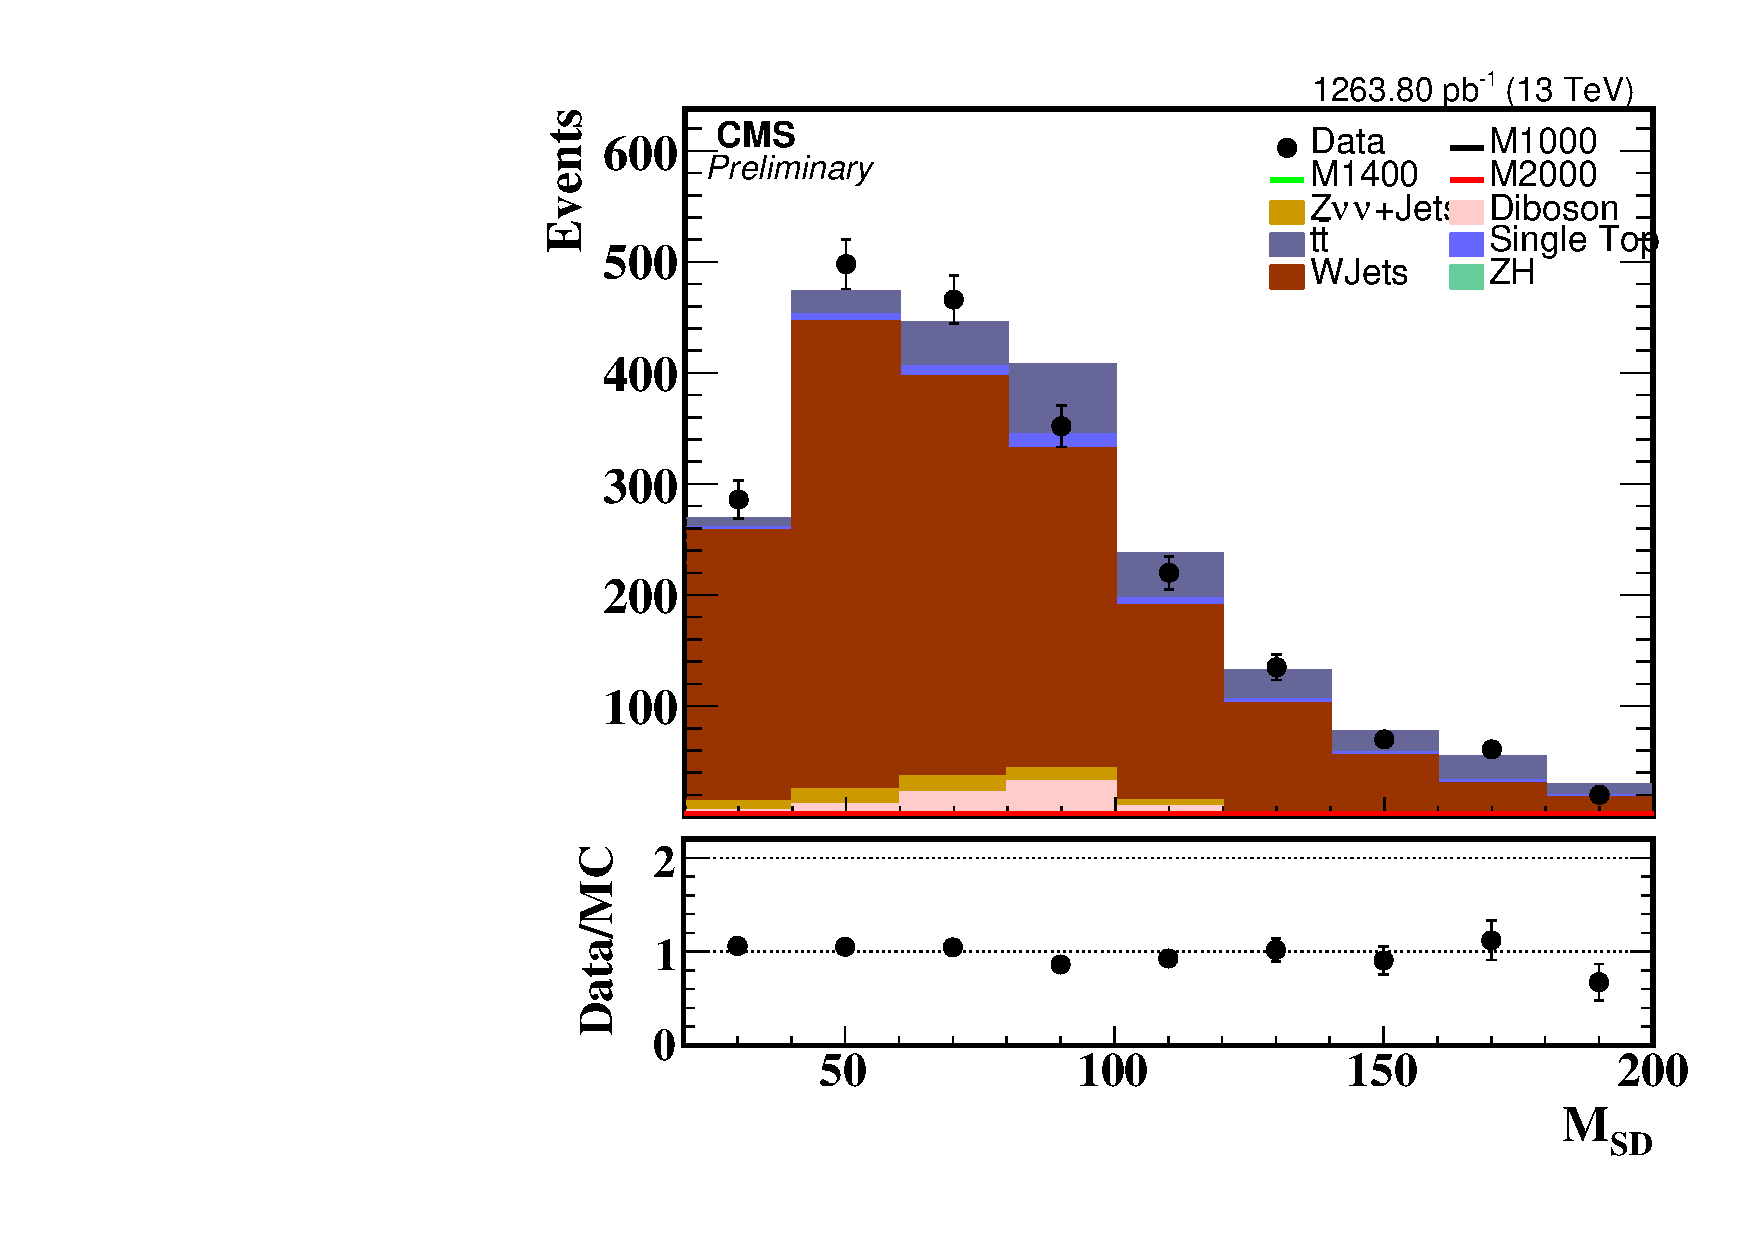
\includegraphics[angle=0,height=0.22\textwidth]{PlotsRaman_VeniceConf30112015/DYPdf/histfacFatJet_WLight_h_Mjj0.pdf}
%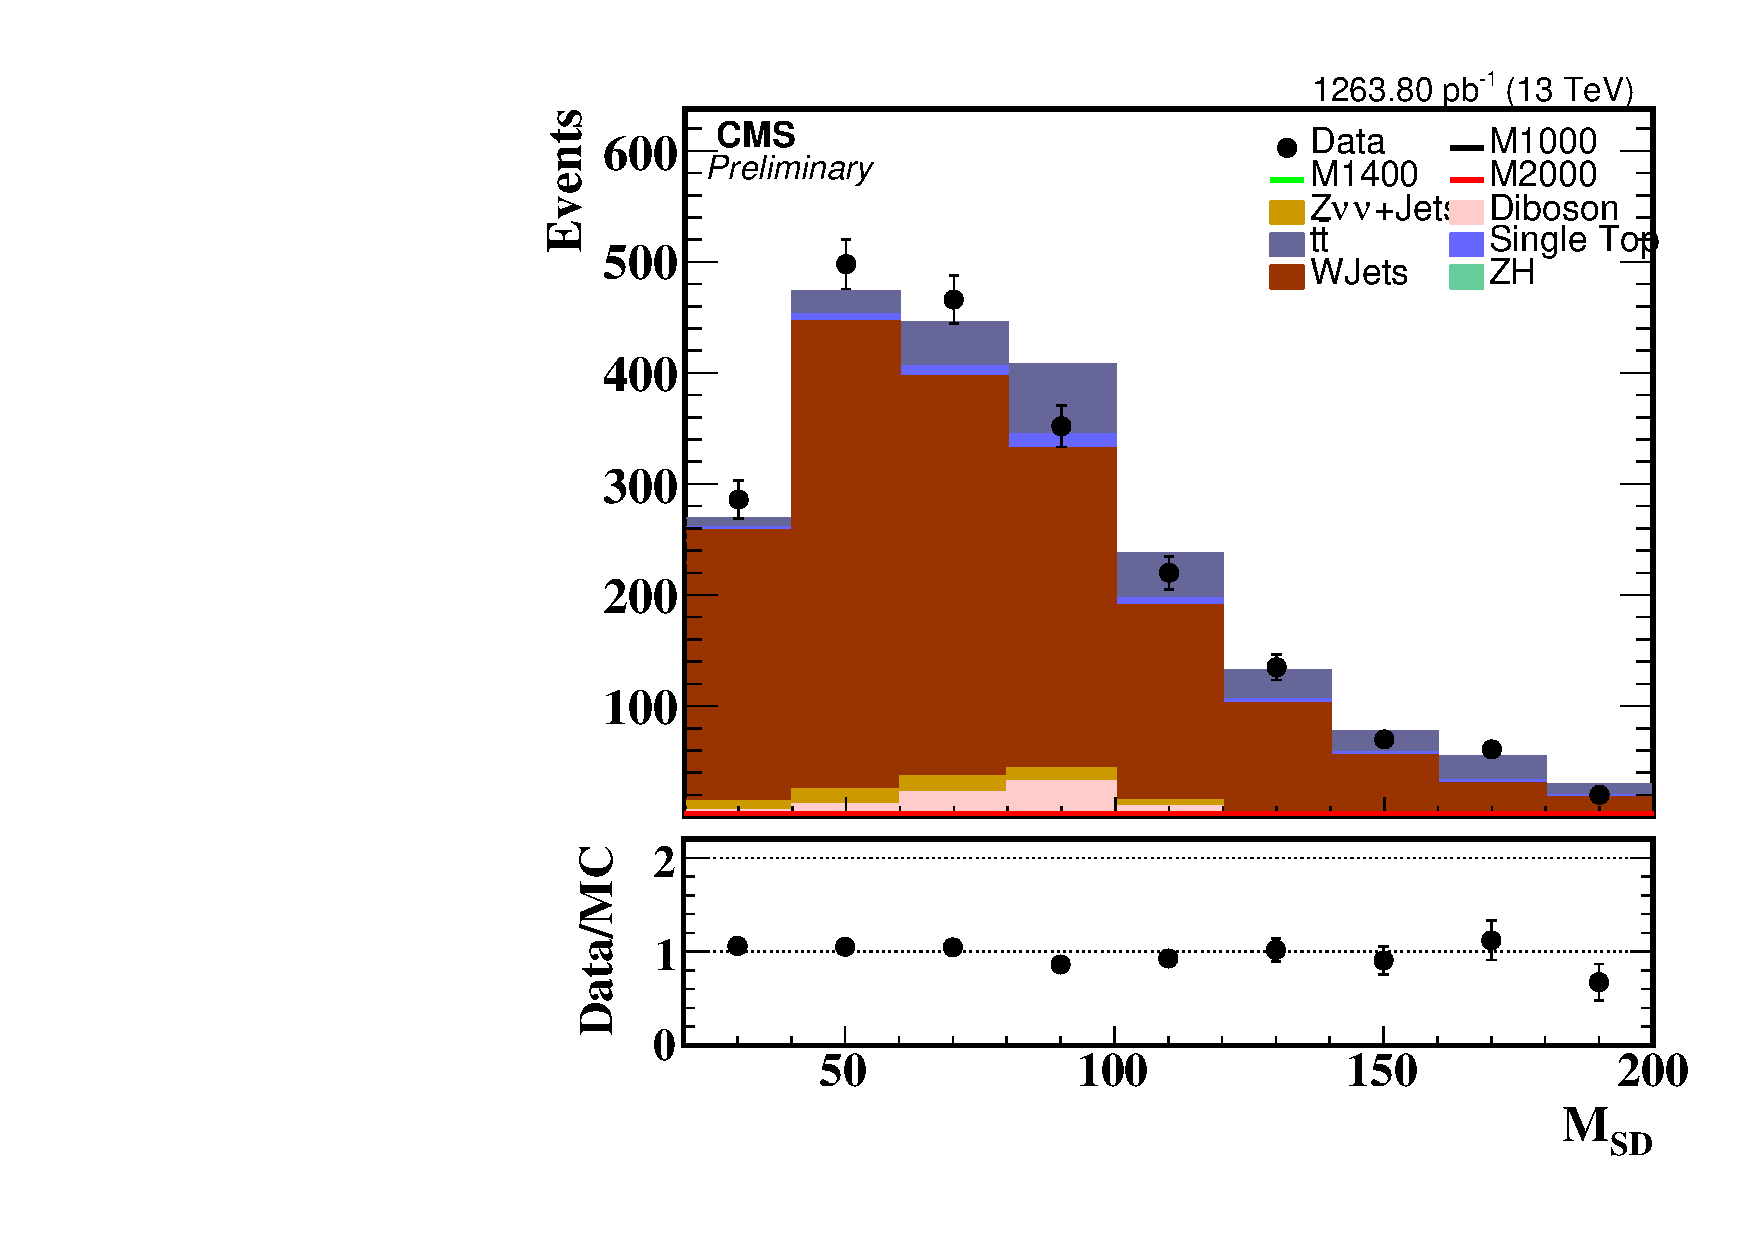
\includegraphics[angle=0,height=0.22\textwidth]{PlotsRaman_VeniceConf30112015/DYPdf/histfacFatJet_WLight_h_Mjj0.pdf}
%\end{center} 
%\end{frame}
%
\end{document}
